\documentclass[a4paper]{article}

\usepackage[english]{babel}
\usepackage[utf8]{inputenc}
\usepackage{amsmath}
\usepackage{amsfonts}
\usepackage{graphicx}
\usepackage{mathtools}
\usepackage[colorinlistoftodos]{todonotes}
\usepackage{tikz}
\usepackage{float}
\usetikzlibrary{arrows.meta}

\newcommand{\bhj}{\widehat{\beta}_j}
\newcommand{\bsj}{\beta^*_j}
\newcommand{\sbsj}{\sigma(\bsj)}

\title{CS 5785 -- Applied Machine Learning -- Lec. 8}

\author{Prof. Nathan Kallus, Cornell Tech}

\date{September 18, 2018}

\begin{document}
\maketitle

\section*{Basics of Inference for the Linear Model}
Inference isn’t the core of this class (the core is making predictive models), however it is a useful tool.\\ \\
Supervised learning algorithm can be thought of as a black box that maps data to a prediction rule ($f^*$).\\

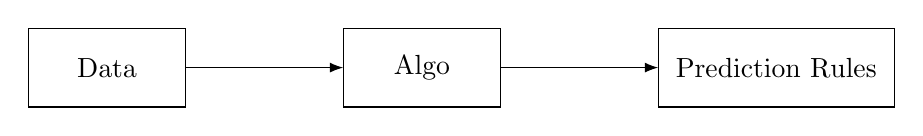
\begin{tikzpicture}
\draw (18, 1) rectangle (20, 2) node[pos=.5] {Data};
\draw [-Latex] (20, 1.5) -- (22, 1.5);
\draw (22,1) rectangle (24,2) node[pos=.5] {Algo};
\draw [-Latex] (24, 1.5) -- (26, 1.5);
\draw (26, 1) rectangle (29, 2) node[pos=.5] {Prediction Rules};
\end{tikzpicture}
\\ \\
OLS is one such algorithm that proceeds as follows:
\begin{align*}
&\hat{f}(X)=\hat{\beta}^T X \\
\mbox{where \hspace{0.5cm}}&\hat{\beta}=(X^T X)^{-1}X^T Y.
\end{align*}
\\
Inference opens up the black box ($\mbox{data} \rightarrow \hat{f}$) and seeks to understand what is going on inside, and what exactly can be learned and generalized. It asks questions like “How does a particular supervised learning algorithm depend on the data, and once we have that understanding, what can we learn from this that generalizes, beyond just the data itself". \\ \\
For example some of the questions we can answer are as follows:
\begin{itemize}
\item How much variance/uncertainty is there in $\hat{\beta}$?
\item How much variance/uncertainty is there in $\hat{f}$(x)?
\item How different is $\hat{f}$ from $f^*$?
\item We know $\hat{f}\ne f^*$, but maybe we can say something about $f^*$ nonetheless?
(i.e. “$f^*$ is like this” and “to what extent is $f^*$ like this?”)
\item How sure are we that a certain variable matters, or does not matter?
\end{itemize}
\bigskip
\begin{figure}
	\centering
	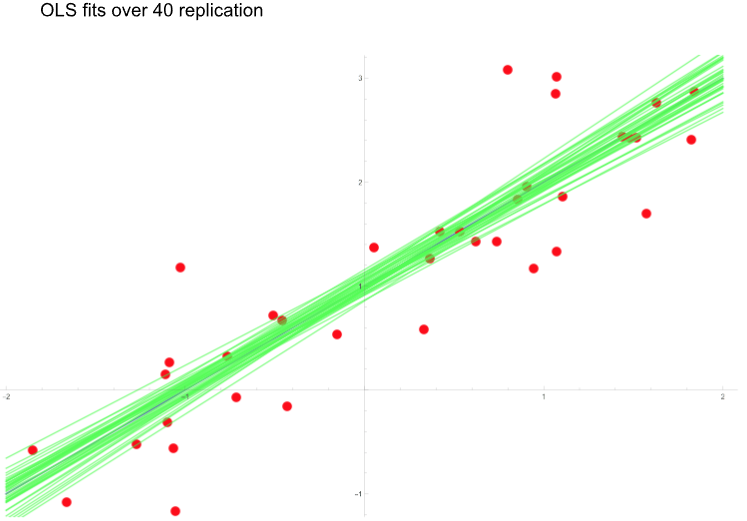
\includegraphics[width=\linewidth]{40_OLS.png}
	\caption{$40$ OLS lines fit to $40$ random draws of data}
    \label{OLS_lines}
\end{figure}
For this lecture we will focus on OLS, and to answer these questions, we must first understand how OLS depends on data. In \textbf{Figure \ref{OLS_lines}}, $40$ points of data were drawn using random, uniformly distributed $x$ and $y=x+1$ with noise of a univariate Gaussian distribution with mean $0$ and variance of $0.5$. \\ \\
Data was drawn randomly $40$ times and a line was fit to the data using OLS each time. In particular, since the data is drawn at random, $\hat{\beta}$ is also random because it depends on the data. Drawing a new set of data is like drawing a new random $\hat{\beta}$.\\ \\
\begin{figure}
	\centering
	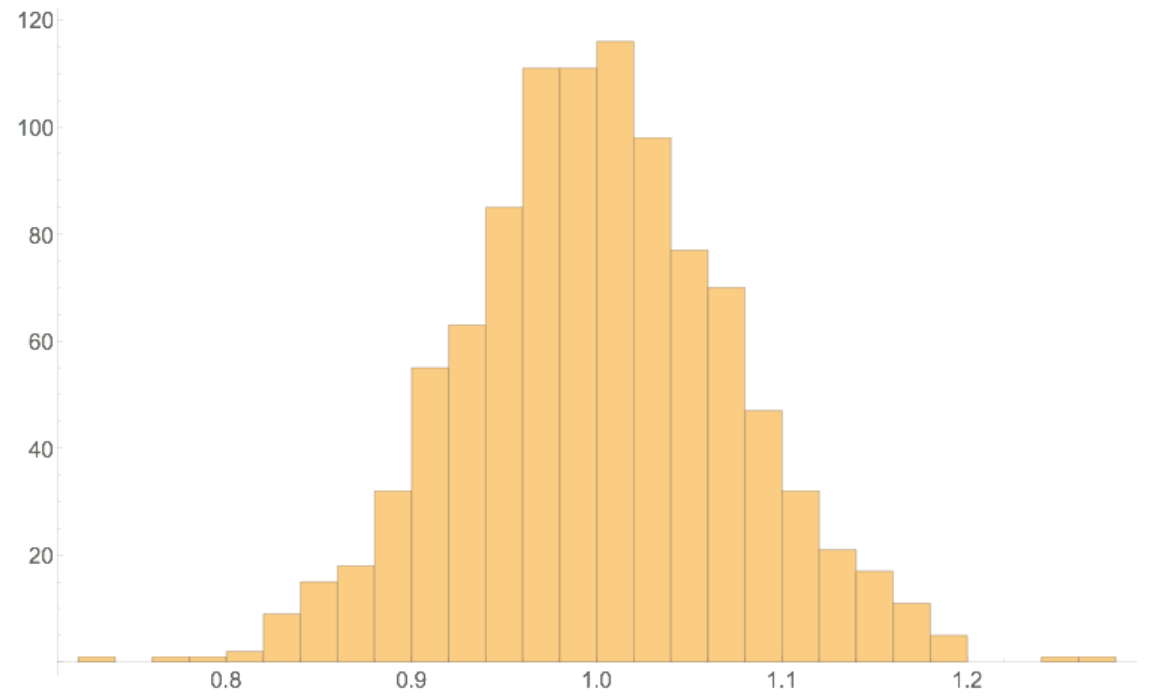
\includegraphics[width=\linewidth]{beta_hist.png}
	\caption{Histogram of $\beta_1$ values over 1000 replications}
    \label{beta_hist}
\end{figure}
\textbf{Figure \ref{beta_hist}} shows a histogram of the slopes (values of $\beta_1$) over 1000 replications.\\ \\
As we know, the correct slope of $f^*$ is 1, and the data is centered on 1, but we have some error. If I get a model with a slope, for example, $\hat{\beta}$ = 0.9, then what can I say about $\beta^*$? Using inference we can make such a statement. \\ \\
Suppose the true model is linear $f^*(x) = \mathbb{E}[Y|X=x] = {\beta^{*}}^T X$\\
And that the errors (deviation of $\hat{Y}$) from for $Y = f^*(x)$ are Gaussian,
\begin{align*}
\epsilon&=y-f^*(x)\sim N(0, \sigma^2), \\
y&=f^*(x)+\epsilon \\
Y&=f^*(X)+E
\end{align*}
\bigskip
Then:
\begin{align*}
\hat{\beta}&=(X^T X)^{-1}X^T Y \\
&=(X^T X)^{-1}(X^T X){\beta}^* + (X^T X)^{-1}E \\
&={\beta}^* + (X^T X)^{-1}E\\
\hat{\beta} - {\beta}^* &= (X^T X)^{-1}E
\end{align*}
where
\begin{align*}
E=(\epsilon_1, \epsilon_2, \cdots, \epsilon_n)^T.
\end{align*}
Note: The second term in line 3 is the error in $\hat{\beta}$.\\ \\
It turns out that $\hat{\beta}$ follows the Multivariate Gaussian Distribution,
\[
\hat{\beta}\sim N(\beta^*, \sigma^2(X^T X)^{-1}),
\]
and $\forall j, k=0,1,2,\cdots,p,j\ne k$,
\begin{align*}
&\mathbb{E}(\hat{\beta}_j)=\beta^*_j,\\
&\mbox{Var}(\hat{\beta}_j)=\sigma^2(X^T X)^{-1}_{jj},\\
&\mbox{Cov}(\hat{\beta}_j,\hat{\beta}_k)=\sigma^2(X^T X)^{-1}_{jk}.
\end{align*}
In particular,
\[
\hat{\beta}_j=N(\beta^*_j,\sigma^2(X^T X)^{-1}_{jj}).
\]
\\
As the number of draws increases (approaching infinity), the distribution approaches Gaussian. If we did $\sim 1,000$ replications we could in fact develop this, unfortunately we don’t often have that number of data sets. Regardless, we know that this will happen, so we do not need $1,000$ replications, however we don’t know the mean and standard deviation of this distribution.\\ \\
So what? First of all, we now know how much uncertainty we have in $\hat{\beta}$:
\[
\sigma_{\hat{\beta}_j}=\sigma \sqrt{(X^TX)^{-1}_{jj}}\\
\]
actually we almost know, but we need 
\begin{align*}
\sigma&=\mathbb{E}[\epsilon^2]\\
&=\mathbb{E}[(Y-\beta^{*T}x)^2]
\end{align*}
\bigskip
We can estimate $\sigma$ in p-dimensions as:
\[
\hat{\sigma} = \frac{1}{n-p-2} \sum^n_{i=1}(Y_i-\hat{\beta}^T x_i)^2
\]
Then, $\beta_j$ has a standard deviation of approximately $\hat{\sigma}\sqrt{(X^TX)^{-1}_{jj}}$\\
Similarly, the prediction at $\hat{F}(x) = \beta^T x$ has a standard deviation  of approximately:
\[
\hat{\sigma}\sqrt{x^T(X^TX)^{-1}x}
\]
This tells us how uncertain we are in our prediction of $\beta^{*T}x$

\section*{}
What does this uncertainty mean? \\
If we were to repeatedly draw a new training dataset of size $n$, and fit OLS to it, the collection of the results we get for the $j^{th}$ coefficient would have such a standard deviation. \\
\\
This quantifies how much uncertainty varies from an algorithm's dependence on the random data.

\begin{equation*}
\widehat{\beta}_j\sim\mathcal{N}\bigg(\beta^*_j,\underbrace{\sigma^2(\mathbb{X}^T\mathbb{X})^{-1}_{jj}}_\text{$\sigma^2(\widehat{\beta}_j)$}\bigg)
\end{equation*}
Where does $\bhj$ fall under the bell curve?\\
Usually in the middle.

\begin{align*}
&\mathbb{P}\bigg(\bsj-z\sigma(\bsj)\leq\bhj\leq\bsj+z\sigma(\bsj)\bigg)\\
&=\mathbb{P}\bigg(-z\leq\underbrace{\frac{\bhj}{\sigma(\bhj)}}_\text{z-score of $\bhj$}-\frac{\bsj}{\sigma(\bhj)}\leq z\bigg)\\&=\mathbb{P}\bigg(-z\leq\mathcal{N}(0,1)\leq z\bigg)
\end{align*}

For $z=1.96\approx 2$, we get that
$$\bsj-z\sigma(\bhj)\leq \bhj	\leq	\bsj+z\sigma(\bhj)$$
happens with probability 95\%\\

Add $-\bsj-\bhj$ and negate

$$\bhj-z\sigma(\bhj)\leq \bsj\leq \bhj+z\sigma(\bhj)$$

with probability 95\%, that is

$$\bsj\in\underbrace{\big[\bhj-z\sigma(\bsj),\bhj+z\sigma(\bsj)\big]}_\text{confidence interval for $\bsj$}$$

\begin{figure}[h]
	\centering
	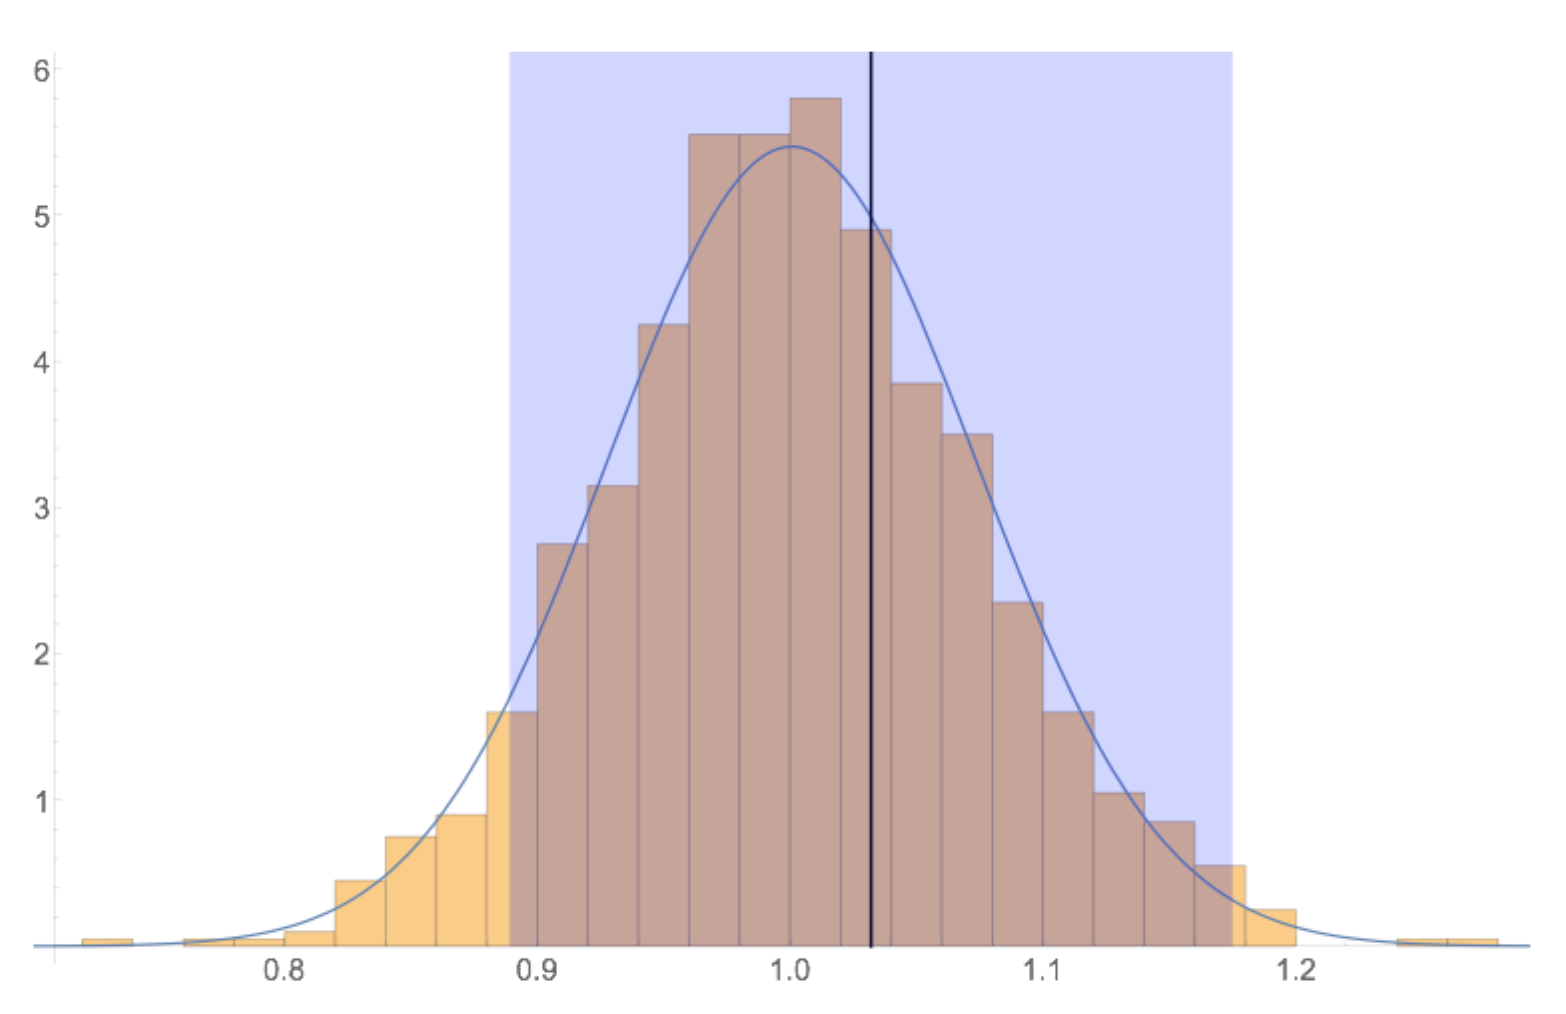
\includegraphics[width=1.0\textwidth]{f2.png}
	\caption{Confidence interval representation for $\bhj$}
\end{figure}

\newpage 
If we knew $\sbsj$, then we know that this interval will contain the unknown $\bsj$ with high probability.
We don't know $\sbsj$, so we estimate it as 

$$\widehat{\sigma}(\bsj)=\widehat{\sigma}\sqrt[]{(\mathbb{X}^T\mathbb{X})^{-1}_{jj}}$$

$\frac{\bhj}{\widehat{\sigma}(\bsj)}$ known as the \underline{t-score} of $\bhj$

Note that going from $\sigma(\bsj)$ to $\widehat{\sigma}(\bsj)$ makes our interval a little to small to cover 95\%. Therefore we need to expand it a bit by using Student T distribution.\\
When n is large, this is about the same, however.

\section*{p-value}
The \underline{p-value} is the largest $p\in[0,1]$ such that the $(1-p)-CI$ contains 0.\\
A way to score how far $\bhj$ is from 0.\\

What does a confidence interval mean?\\
The probability 95\% is over random new draws of data.\\
I.e. given the data \& interval, it's not that $\bsj$ is random and may be in the interval with probability 95\%. \\
Rather, it's $\bhj$ that's random.

How to implement in code?
\begin{figure}[H]
	\centering
	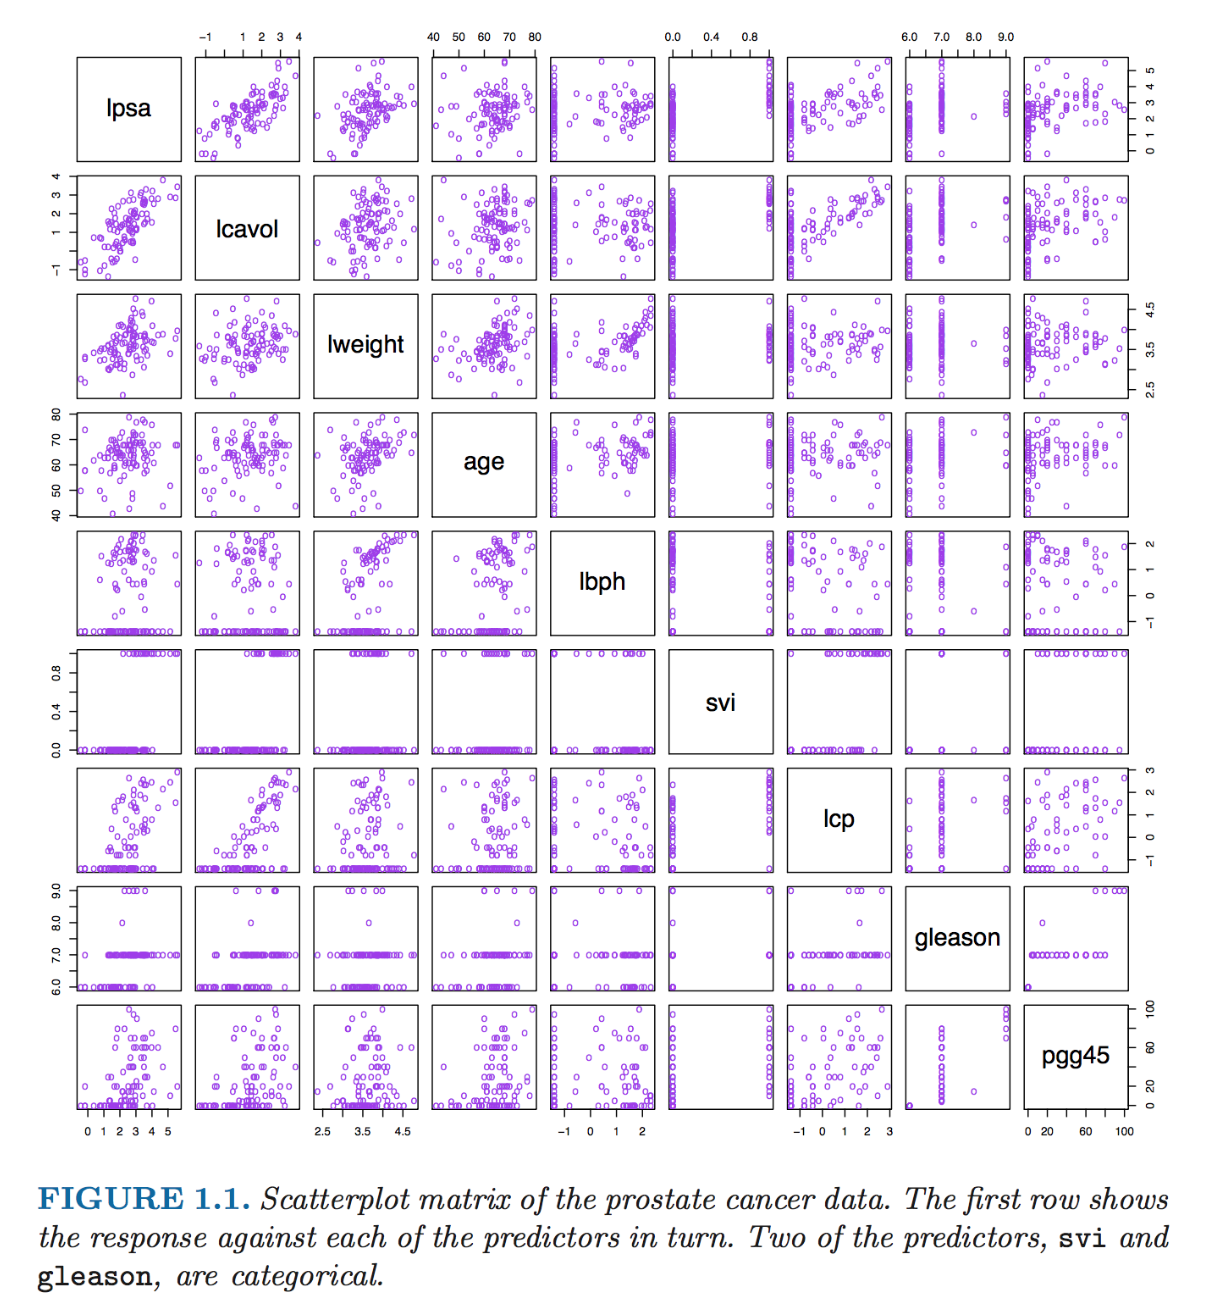
\includegraphics[width=.8\textwidth]{f3.png}
	\caption{Scatterplot Matrix}
\end{figure}
\begin{figure}[H]
	\centering
	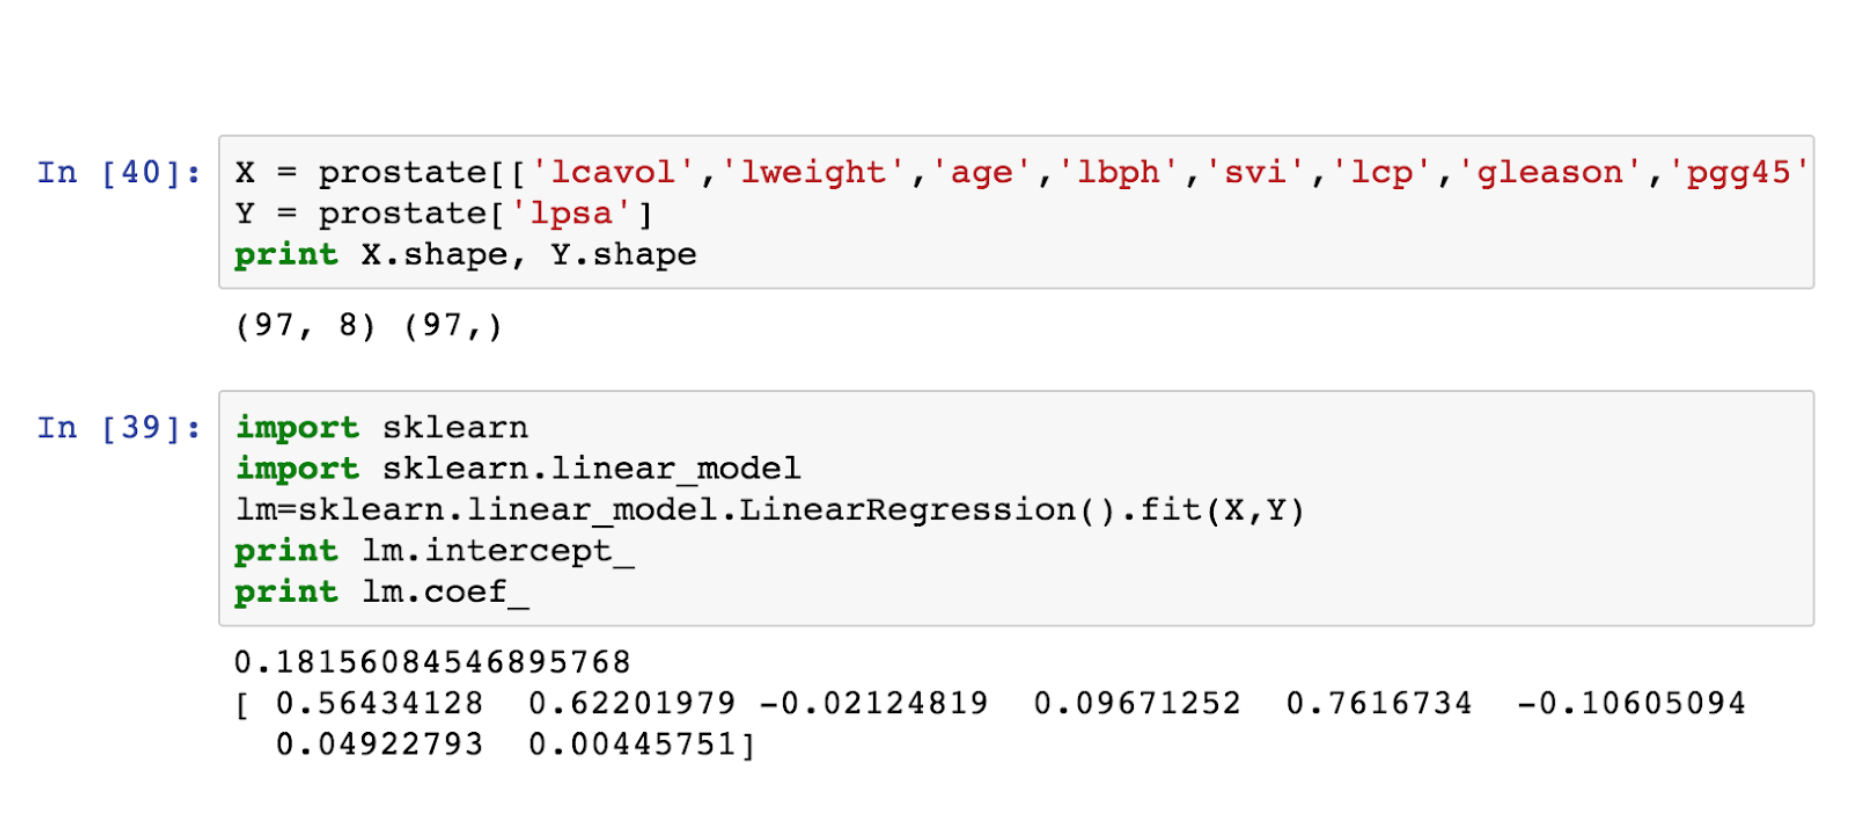
\includegraphics[width=.8\textwidth]{f4.png}
	\caption{Code example implementation}
\end{figure}
\begin{figure}[H]
	\centering
	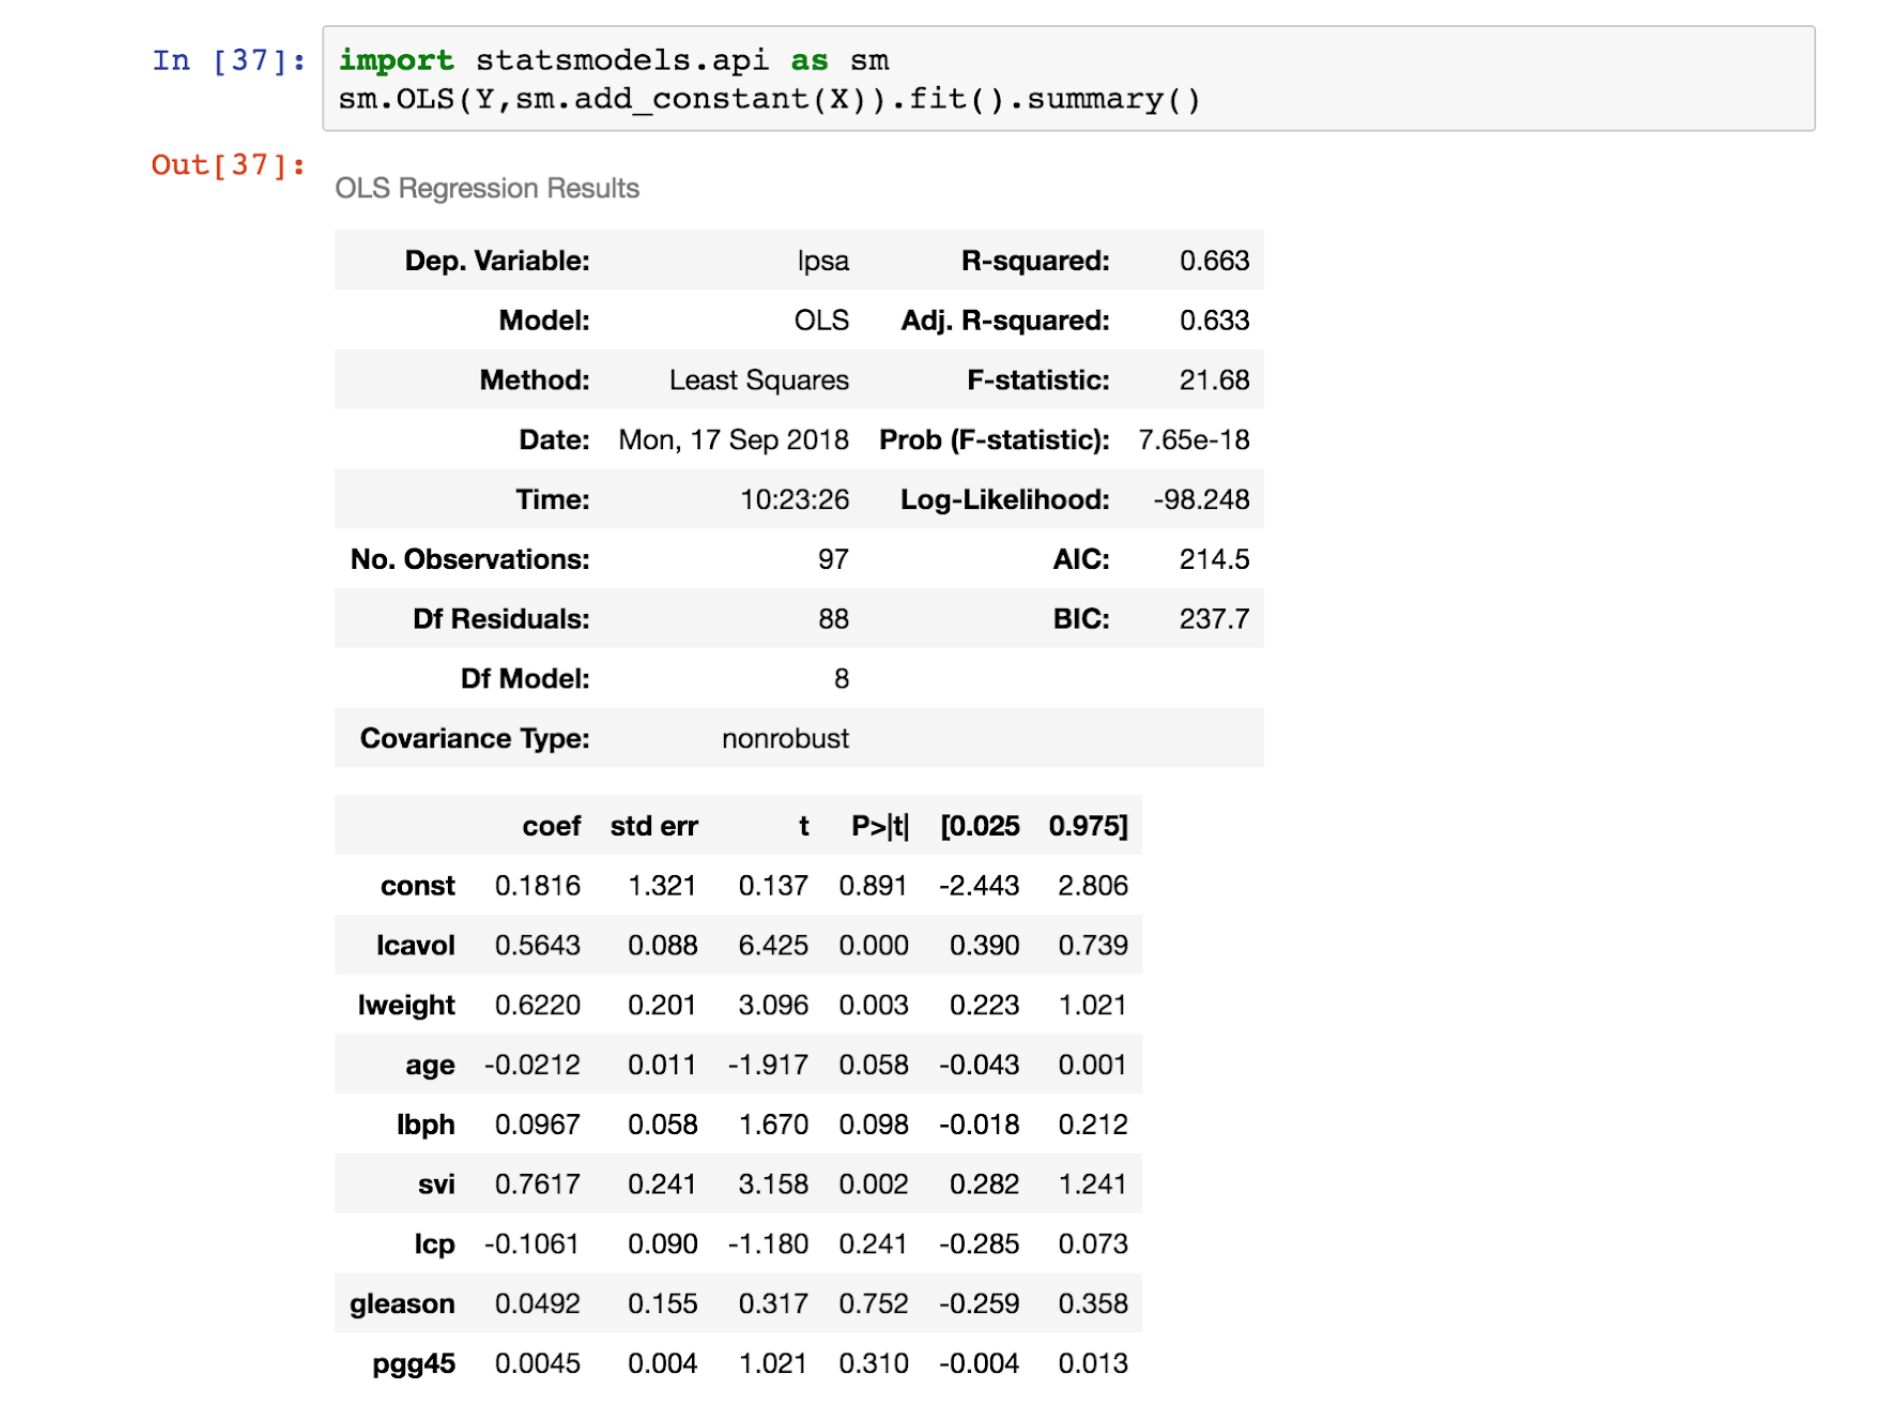
\includegraphics[width=.8\textwidth]{f5.png}
	\caption{Statistic summary}
\end{figure}

\section*{Beyond OLS}
We are only covering the basics of inference - just enough to understand confidence intervals.\\
A few things to be aware of (mostly without explanation):\\
\begin{itemize}
	\item What if $\epsilon$ is not normally distributed?\\
    	Mostly OK, as long as n is moderately sized relatively to p.
        We shouldn't worry about this.
    \item What if $f^*$ is not linear?\\
       The inference is really on $f^*$ best linear approximation. It makes sense if $f^*$ is almost linear.
    \item What about linear regression?\\
       Proceeds mostly the same. Most packages for linear regression (sklearn excluded) will report p-values and confidence 			intervals for coefficients.
    \item What about shrinkage and subset selection?\\
    	Won't work out of the box (for inference on coefficients)... Advanced topic.
    \item What about kNN, neural networks etc?\\
    	Can make inference on predictions $\widehat{f}(x)$. Hard to do on the model itself.
\end{itemize}


\end{document}